%<*manuscript|acmsmall|acmsmall-submission|acmlarge|acmtog|sigconf|authordraft|sigplan|sigchi|sigchi-a|acmsmall-conf>
%% 
%% The first command in your LaTeX source must be the \documentclass command.
%<manuscript>\documentclass[manuscript,screen,review]{acmart}
%<acmsmall|acmsmall-conf>\documentclass[acmsmall]{acmart}
%<acmsmall-submission>\documentclass[acmsmall,screen,review]{acmart}
%<acmlarge>\documentclass[acmlarge]{acmart}
%<acmtog>\documentclass[acmtog]{acmart}
%<sigconf>\documentclass[sigconf]{acmart}
%<authordraft>\documentclass[sigconf,authordraft]{acmart}
%<sigplan>\documentclass[sigplan,screen]{acmart}
%<sigchi>\documentclass[sigchi]{acmart}
%<sigchi-a>\documentclass[sigchi-a, nonacm]{acmart}

%%
%% \BibTeX command to typeset BibTeX logo in the docs
\AtBeginDocument{%
  \providecommand\BibTeX{{%
    \normalfont B\kern-0.5em{\scshape i\kern-0.25em b}\kern-0.8em\TeX}}}

%% Rights management information.  This information is sent to you
%% when you complete the rights form.  These commands have SAMPLE
%% values in them; it is your responsibility as an author to replace
%% the commands and values with those provided to you when you
%% complete the rights form.
%
\setcopyright{acmcopyright}
\copyrightyear{2018}
\acmYear{2018}
\acmDOI{10.1145/1122445.1122456}

%</manuscript|acmsmall|acmsmall-submission|acmlarge|acmtog|sigconf|authordraft|sigplan|sigchi|sigchi-a|acmsmall-conf>
%<*manuscript|sigconf|authordraft|sigplan|sigchi|sigchi-a|acmsmall-conf>
%% These commands are for a PROCEEDINGS abstract or paper.
\acmConference[ICPP '21]{ICPP '21: 50th International Conference on Parallel Processing}{August 09--12, 2021}{Chicago, IL} 
\acmBooktitle{ICPP '21: 50th International Conference on Parallel Processing,
  August 09--12, 2021} 
\acmPrice{15.00}
\acmISBN{978-1-4503-XXXX-X/18/06}
%</manuscript|sigconf|authordraft|sigplan|sigchi|sigchi-a|acmsmall-conf>

%<*acmsmall|acmsmall-submission|acmlarge|acmtog>
%%
%% These commands are for a JOURNAL article.
%<acmsmall|acmsmall-submission>\acmJournal{JACM}
%<acmlarge>\acmJournal{POMACS}
%<acmtog>\acmJournal{TOG}
\acmVolume{37}
\acmNumber{4}
\acmArticle{111}
\acmMonth{8}
%</acmsmall|acmsmall-submission|acmlarge|acmtog>
%<*manuscript|acmsmall|acmsmall-submission|acmlarge|acmtog|sigconf|authordraft|sigplan|sigchi|sigchi-a|acmsmall-conf>


%%
%% Submission ID. 
%% Use this when submitting an article to a sponsored event. You'll
%% receive a unique submission ID from the organizers
%% of the event, and this ID should be used as the parameter to this command.
%%\acmSubmissionID{123-A56-BU3}


%%
%% The majority of ACM publications use numbered citations and
%% references.  The command \citestyle{authoryear} switches to the
%% "author year" style.
%%
%% If you are preparing content for an event
%% sponsored by ACM SIGGRAPH, you must use the "author year" style of
%% citations and references.
%<!acmtog>%% Uncommenting 
%<!acmtog>%% the next command will enable that style.
%<!acmtog>%%\citestyle{acmauthoryear}
%<acmtog>\citestyle{acmauthoryear}

\usepackage{graphicx}
\usepackage{tikz}
\usepackage{rotating}
\usepackage{algorithm}
\usepackage[noend]{algpseudocode}

\usetikzlibrary{decorations.pathreplacing,shapes,arrows,positioning}

%%
%% end of the preamble, start of the body of the document source.
\begin{document}

%%
%% The "title" command has an optional parameter,
%% allowing the author to define a "short title" to be used in page headers.
\title{Compiling Files in Parallel: A Study with GCC}

%%
%% The "author" command and its associated commands are used to define
%% the authors and their affiliations.
%% Of note is the shared affiliation of the first two authors, and the
%% "authornote" and "authornotemark" commands 
%% used to denote shared contribution to the research.
\author{Giuliano Belianssi}
\email{giuliano.belinassi@usp.br}
\orcid{1234-5678-9012}
\author{Alfredo Goldman}
\email{gold@ime.usp.br}
\affiliation{%
  \institution{Institute of Mathematics and Statistics}
  \streetaddress{Rua do Matão, 1010}
  \city{São Paulo}
  \state{São Paulo}
  \country{Brazil}
  \postcode{05508-060}
}

\author{Richard Biener}
\affiliation{%
  \institution{SUSE Labs}
  \streetaddress{Nürnberg 90409}
  \city{Nürnberg}
  \country{Germany}}
\email{rguenther@suse.de}

\author{Jan Hubi\v cka}
\affiliation{%
  \institution{Charles University}
  \streetaddress{CMalostransk én ám. 25}
  \city{Praha}
  \country{Czech Republic}}
\email{hubicka@ucw.cz}


%%
%% By default, the full list of authors will be used in the page
%% headers. Often, this list is too long, and will overlap 
%% other information printed in the page headers. This command allows
%% the author to define a more concise list 
%% of authors' names for this purpose.
\renewcommand{\shortauthors}{Belinassi et al.}

%%
%% The abstract is a short summary of the work to be presented in the
%% article. 
\begin{abstract}
Processors are becoming increasingly parallel, but compiling software has so
far been a task parallelizable only by per file granularity. To improve
this, we propose a method feasible to implement
in commercial compilers for parallel single file compilation, using simple
modifications in the Link Time Optimization (LTO) engine; which we show by
implementing a custom partitioner in GCC. This method resulted in a 35\% speedup when
self-compiling GCC when compared to \texttt{make -j} only parallelism, and speedups
ranging from $0.7\times$ to $3.5\times$ when compiling individual files. 
We also explain why the adoption of our proposed method is still compatible
with the Reproducible Builds project.
\end{abstract}

%%
%% The code below is generated by the tool at http://dl.acm.org/ccs.cfm.
%% Please copy and paste the code instead of the example below.
%%
\begin{CCSXML}
<ccs2012>
<concept>
<concept_id>10011007.10011006.10011041</concept_id>
<concept_desc>Software and its engineering~Compilers</concept_desc>
<concept_significance>500</concept_significance>
</concept>
<concept>
<concept_id>10010147.10010169.10010170</concept_id>
<concept_desc>Computing methodologies~Parallel algorithms</concept_desc>
<concept_significance>500</concept_significance>
</concept>
</ccs2012>

\end{CCSXML}

\ccsdesc[500]{Software and its Engineering~Compilers}
\ccsdesc[300]{Computer methodologies~Parallel algorithms}

%%
%% Keywords. The author(s) should pick words that accurately describe
%% the work being presented. Separate the keywords with commas.
\keywords{Compilers, Parallel Compilation, Link Time Optimization, LTO, GCC}

%</manuscript|acmsmall|acmsmall-submission|acmlarge|acmtog|sigconf|authordraft|sigplan|sigchi|sigchi-a|acmsmall-conf>
%<*sigconf|authordraft|sigplan|acmsmall-conf>
%% A "teaser" image appears between the author and affiliation
%% information and the body of the document, and typically spans the
%% page.
%%\begin{teaserfigure}
%%  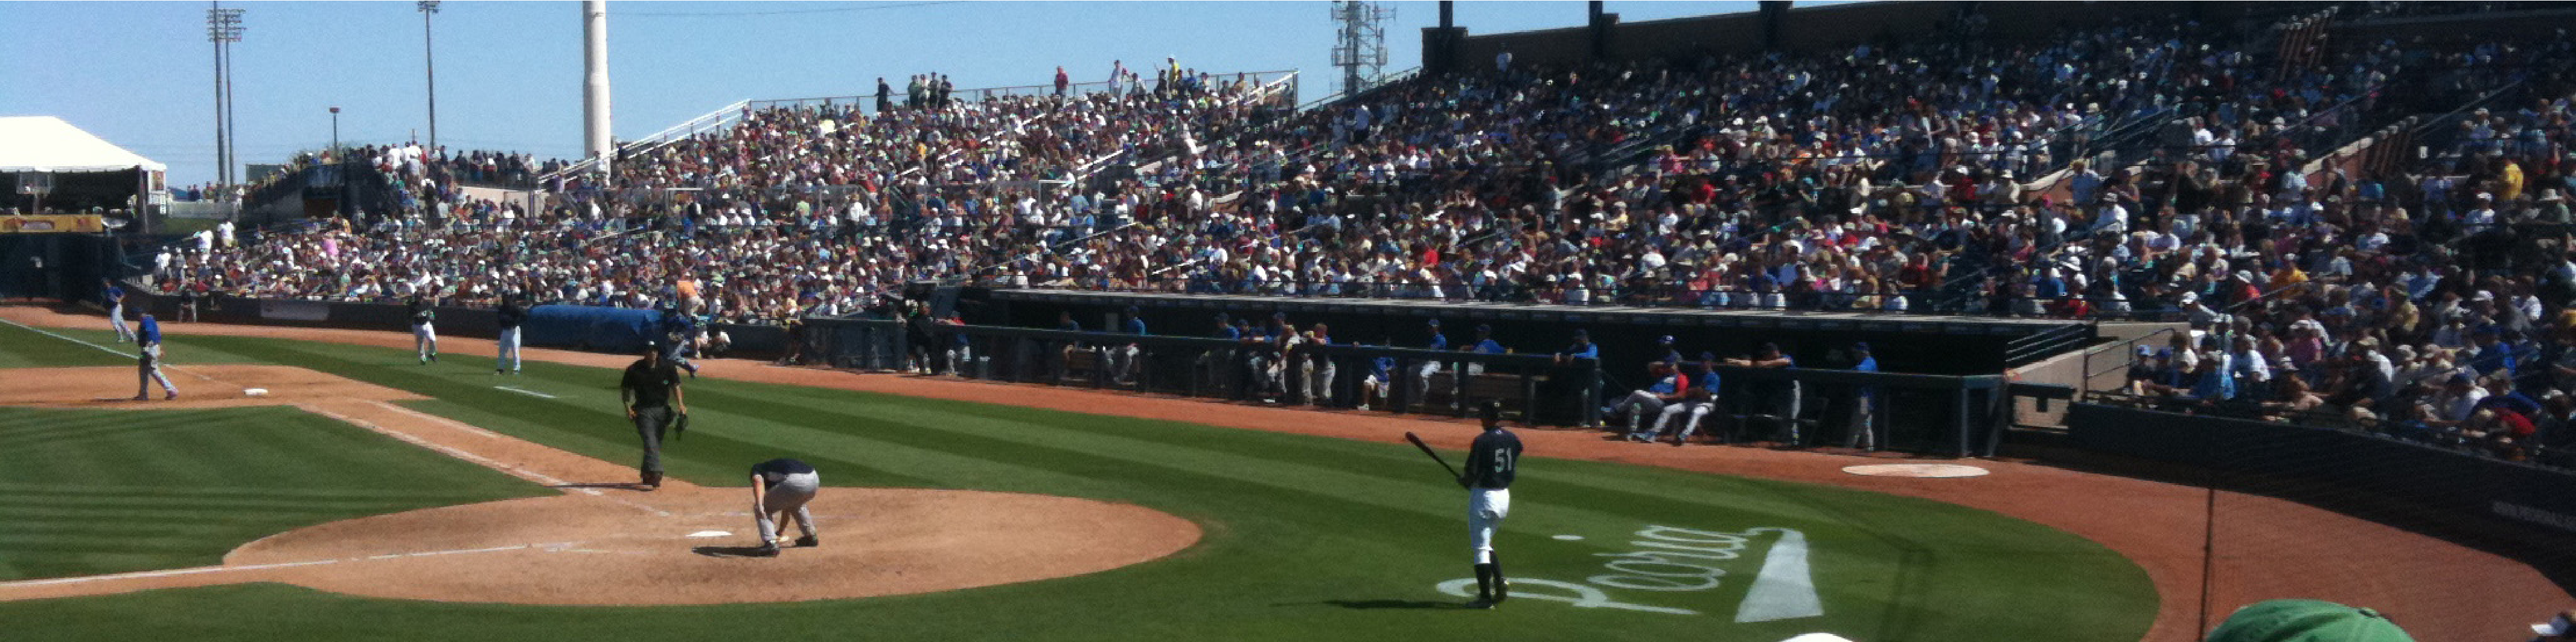
\includegraphics[width=\textwidth]{sampleteaser}
%%  \caption{Seattle Mariners at Spring Training, 2010.}
%%  \Description{Enjoying the baseball game from the third-base
%%  seats. Ichiro Suzuki preparing to bat.} 
%%  \label{fig:teaser}
%%\end{teaserfigure}
%</sigconf|authordraft|sigplan|acmsmall-conf>
%<*manuscript|acmsmall|acmsmall-submission|acmlarge|acmtog|sigconf|authordraft|sigplan|sigchi|sigchi-a|acmsmall-conf>

%%
%% This command processes the author and affiliation and title
%% information and builds the first part of the formatted document.
\maketitle

\section{Introduction}

The recent advances in both technological and computational fields induced an
increasingly faster expansion of software ecosystems. Developers create new
programs to supply the needs of the most diverse domains by coding new websites
in scripting languages, creating standalone desktop applications, adding new
functionalities to an operating system, and so on. Regardless of the reason
behind the development of them, it is true that their code will be, at some
point, transformed into machine language by a compiler or assembler, even if an
interpreter executes it.

Compilers are enormous programs, largely adopted by industry and academia, where
a great effort has been employed to produce efficient code --
but without any sacrifice in correctness --. There are huge projects destined
to develop and improve them, such as the GNU Compiler Collections
(GCC)\footnote{https://gcc.gnu.org/} and LLVM\footnote{https://llvm.org/}, capable
of translating several languages such as C, C++, and Fortran, to machine language.

GCC was started by Richard Stallman, with the first public release in March of
1987, supporting only the C language and targeting several architectures
\cite{gcc-first-ver}. Today, GCC is a multinational collaboration
project, with hundreds of thousands of lines of code, and perhaps the most used C/C++
compiler in the Linux ecosystem.

GCC was initially designed to compile programs one file at a time, meaning
that it could not allow global cross-file optimizations because the compiler
never had the opportunity to analyze the program as a whole. This scenario
changed when Link Time Optimization (LTO) was proposed \cite{gcc-lto,whoprgoogle} and
implemented \cite{glek2010optimizing}. GCC supports LTO by using
\texttt{-flto}. Part of the LTO engine has already been parallelized, which
inspired this work.

The main contribution of this work is to answer the question about how can we modify an
industrial scale compiler to compile single files in parallel. We address
that by reusing the already-existing LTO engine in it (in this
case, GCC) for partitioning the single file Translation Unit (TU) after the
Interprocedural Analysis (IPA) has been decided, and we proceed compiling
each partition individually, in parallel. IPA includes only interprocedural
optimizations, which requires interactions among distinct functions to optimize
(\emph{e.g.} inliner). There is already a way to instruct
the LTO engine to partition a single file TU by using the flags
\texttt{-flto } \texttt{-flinker-output=nolto-rel}, but with phony object creation
overhead and no guarantee of correct name clash resolution, as discussed
in Section \ref{sec:name_clash_resolution}.

We present the previous efforts in compiling a single file in parallel, as well
as an introduction to LTO in Section \ref{sec:related}.  Then, discuss the idea
that motivated the development of this feature on Section \ref{sec:profiling},
reproducing previous profiling experiments on GCC and computing an
approximation about the best speedup archivable by our methods; to finally
present our proposal on section Section \ref{sec:work}, as well as presenting
some internal details of GCC. We then show how we ensured that our
modifications are correct in Section \ref{sec:methods}; and finally, we present
our results in Section \ref{sec:results} with a discussion about our findings and
observations when running the experiments. In the end, we discuss how to improve
from this paper in Section \ref{sec:future_works}.


\section{Related Works} \label{sec:related}

Parallel Compilation includes parsing (parallel or not), how to perform
analysis, optimization, and code translation in parallel.  Parsing can be
described as building a machine to decide if an input string is a member of a
certain language or not, creating the Abstract Syntax Tree in the process by
logging the used derivation rules.

Parallel Parsing dates back to 1970. Lincoln \cite{Lincoln:1970:PPT:987475.987478}
explored how to use the vectorial registers in the (so far)
STAR-100 supercomputer for lexical analysis. Fischer
\cite{fischer1975parsing} gives a detailed theoretical study, proving
several concurrent parsing techniques for the LR($k$) family.
The parser proceeds by breaking the input into several arbitrary parts, and running a
serial parser on each of them. Then the algorithm tries to
recover the stack of each noninitial parser by constructing a set of
possible states, for which there are 5 possible cases. However, in case
of an error, the parser result should be discarded, and therefore a lot
of work will be done in vain when comparing with the sequential version.

Fowler and Joshua \cite{fowler2009parallel} described how to parallelize Earley
and Packrat methods. For the former, the authors partition the Earley sets into
sub-blocks and run each block in parallel. For solving the dependency across
the blocks, the authors propose a way to speculate additional items into the
parser, which are not produced by the serial algorithm. For Packrat, the authors
propose a message passing mechanism.  The input is divided into parts, and each
part is assigned to a worker thread. Each thread speculates until the
thread on its left has finished parsing, and send the synthesized starting
symbol to the thread on its right. The authors managed a speedup of $5.5\times$
in Earley, and $2.5\times$ in Packrat.

Still on Packrat methods, Dubroy and Warth \cite{dubroy2017incremental} show
how to implement an incremental Pacrkat to avoids reparsing the entire input
on modifications. The authors achieve this by recording all its
intermediate results in a parsing table and modify the parsing program to reload
this table when invoked. They further showed that their method does not require
any modification to the original grammar, and their method requires only
up to $11.7\%$ of extra memory when compared to the original parser. Authors
claim a reduction from $23.7ms$ to $6.2ms$ on reparsing a 279Kb input string.

Barenghi \textit{et al.} \cite{Barenghi:2015:PPM:2839536.2840146} explore
some properties of Operator Precedence Grammars to construct a Yacc-like
parser constructor named PAPAGENO, which generates parallel parsers. The
authors described precedence grammars for Lua and JSON, which they used in
their tests to get a speedup of up to $5.5\times$ when compared to a parser
generated by GNU Bison.

As for parallel compilation \textit{de facto}, works dates back from 1988.
Vandevoorde \cite{vandevoorde1988parallel} worked on a C compiler, and Wortman
and Junkin \cite{wortman1992} worked on a Modula-2+ compiler.  The former
assumes that every function declaration is in the file headers, and implements
per-function and per-statement parallel compilation. The latter implements only
per-function parallelism.  Speedups ranged from $1.5\times$ to $6\times$ on a
multicore MicroVAX II machine. None of these papers discuss optimization, and
they concentrate on (today's perspective) non-optimizer compilers, which are not
the case of GCC.

Lattner \emph{et al.} proposed MLIR, an Intermediate Representation (IR) which
aims to unify several Machine Learning frameworks and compilers IR \cite{mlir}.
Its design also includes support to multithreaded compilation by supporting
concurrent transversal and modification of the IR.

There has been an attempt of parallelizing GCC by threading the GIMPLE
intraprocedural pass manager \cite{bernardino2020improving}, which only
requires information contained inside the function's body (\textit{e.g.}
vectorization). The authors managed a speedup of up to $3.35\times$ to this
compilation stage, and up to $1.88\times$ in total compilation of a file when
extending this technique to the RTL passes.

Panchenko \textit{et.al.} \cite{panchenko2021lightning} presented Lightning
BOLT, a compiler that reads already compiled binaries and outputs an optimized
version of them. The authors present a list of passes in which Lightning BOLT
runs in parallel and briefly explain how they parallelized them. They include
Control-Flow Graph Construction, Local Optimizations, Identical Code Folding,
Frame optimizations, and Shrink Wrapping running in parallel. Speedups ranged
up to $1.56\times$ when compared to the sequential version.

\subsection{Link Time Optimization (LTO)} \label{lto_section}

Compilation usually uses the following scheme: a compiler consumes a source file,
generating an assembly file as output. This file is then assembled into an object file
and later linked with the remaining objects file to compose an executable or a library.
Figure \ref{fig:gnu_toolchain} illustrates this process for a single file. In this paper,
we call this method the \emph{classical compilation} scheme.

\begin{figure}
\tikzstyle{block} = [rectangle, draw, fill=white,
    text width=6em, text centered, rounded corners, node distance=4.5cm, auto, minimum height=3em]
\tikzstyle{line} = [draw, -latex]
\tikzstyle{cloud} = [draw, ellipse,fill=white, node distance=2cm,
    minimum height=2em]
%\makebox[\textwidth][c]{
\scalebox{0.8}{
\begin{tikzpicture}[node distance = 1cm, auto]
    % Place nodes
    \node [block]                      (cc1) {Compiler \\ (cc1)};
    \node [block, right of = cc1]      (as) {Assembler\\(as)};
    \node [block, right of = as]       (ld) {Linker};
    \coordinate [above= of cc1]          (fonte);
    \coordinate [above= of ld]    (bin);

    % Draw edges
    \draw[->]    (cc1.east)    -- (as.west)       node[midway, above] {Assembler File};
    \draw[->]    (cc1.east)    -- (as.west)       node[midway, below] {(.s)};
    \draw[->]    (as.east)     -- (ld.west)       node[midway, above] {Object File};
    \draw[->]    (as.east)     -- (ld.west)       node[midway, below] {(.o)};
    \draw[->]    (fonte.south)  -- (cc1.north)      node[pos=0, above] {Source File};
   %\draw[->]    (fonte.south)  -- (cc1.north)      node[pos=0, below] {(.c)};
    \draw[->]    (ld.north)     -- (bin.south)      node[pos=1, above] {Executable};
\end{tikzpicture}
}
%}%
\caption{GCC Compiling a .c file in \emph{classical compilation} mode}
\label{fig:gnu_toolchain}
\end{figure}

The issue around this scheme is that it can only optimize with
the information found in its Translation Unit (TU) because it can not see the body
content of other files' functions. A TU is the
entire content of a source file (a .c file in C) plus all its headers.

As an answer to this, LTO allows cross-module optimizations by
postponing optimizations and final translation to a linker wrapper. There, the entire
program can be loaded by the compiler (but more often, just some sort of summary)
as a single, big TU, and optimizations can be decided globally,
as now it has access to the internals of other modules. LTO is divided into
three steps \cite{whoprgoogle,glek2010optimizing}:
\begin{itemize}
\item LGEN (\textit{Local Generation}): each module is translated to an IR and
written to disk in phony object files. These objects are \emph{phony} because
they do not contain assembly code. This step runs serially on the input file
(\textit{i.e.} in parallel to the files in the project).

\item WPA (\textit{Whole Program Analysis}): load all translated modules,
merges all TUs into one, and analyzes the program globally. After that, it
generates an \emph{optimization summary} for the program and partitioned this
global TU for the next stage. This analysis runs sequentially to the entire
project.

\item LTRANS (\textit{Local Transformations}): apply the transformations generated by
WPA to each partition, which will generate its own object file. This stage runs in
parallel.
\end{itemize}

This process is sketched in Figure \ref{fig:whopr_build}, where the linker
wrapper is represented by \textit{collect2}, which firstly launch \textit{lto1}
in WPA mode, and the second time it finally launches \textit{ld}. This process
can be seen by launching gcc with \texttt{-flto -v}.

\begin{figure}
\tikzstyle{block} = [rectangle, draw, fill=white,
    text width=6em, text centered, rounded corners, node distance=1cm and 0.5cm, minimum height=2em]
\tikzstyle{line} = [draw, -latex]
%\makebox[\textwidth][c]{

\scalebox{0.8}{
\begin{tikzpicture}[node distance = 3cm, auto]
    % Place nodes
    \node [block]              (fonte1) {source1.c};
    \node [block, right= of fonte1]        (fonte2) {source2.cpp};
    \node [block, right= of fonte2]        (fonte3) {source3.f90};
    \node [block, above= of fonte2]         (make)   {Makefile};

    \node [block, below= of fonte1]        (gcc)      {gcc};
    \node [block, below= of fonte2]        (g++)      {g++};
    \node [block, below= of fonte3]        (gfortran) {gfortran};

    \node [block, below= of gcc]           (objeto1) {obj1.o};
    \node [block, below= of g++]           (objeto2) {obj2.o};
    \node [block, below= of gfortran]      (objeto3) {obj3.o};

    \node [block, below= of objeto2]       (gcc_lto) {collect2 (lto1)};

    \node [block, below= of gcc_lto]       (gcc_wpa) {gcc\_wpa};

    \node [block, below= of gcc_wpa]   (gcc_ltrans2) {gcc\_ltrans};
    \node [block, left= of gcc_ltrans2]            (gcc_ltrans1) {gcc\_ltrans};
    \node [block, right= of gcc_ltrans2]   (gcc_ltrans3) {gcc\_ltrans};

    \coordinate[below= of gcc_wpa]            (c2);


    \node [block, below= of gcc_ltrans1]   (obj1) {obj1.o};
    \node [block, below= of gcc_ltrans2]   (obj2) {obj2.o};
    \node [block, below= of gcc_ltrans3]   (obj3) {obj3.o};

    \node [block, below=of obj2]   (ld) {collect2 (LD)};

	\node [block, below=of ld]   (bin) {Binary};

    % Draw edges
    \draw[->]    ([xshift=-0.7em] make.south)   -- (fonte1.north);
    \draw[->]    (make.south)   -- (fonte2.north);
    \draw[->]    ([xshift=+0.7em] make.south)   -- (fonte3.north);

    \draw[->]    (fonte1.south)   -- (gcc.north);
    \draw[->]    (fonte2.south)   -- (g++.north);
    \draw[->]    (fonte3.south)   -- (gfortran.north);

    \draw[->]    (gcc.south)   -- (objeto1.north);
    \draw[->]    (g++.south)   -- (objeto2.north);
    \draw[->]    (gfortran.south)   -- (objeto3.north);

    \draw[->]    (objeto1.south)   -- ([xshift=-0.7em]gcc_lto.north);
    \draw[->]    (objeto2.south)   -- (gcc_lto.north);
    \draw[->]    (objeto3.south)   -- ([xshift=+0.7em]gcc_lto.north);

    \draw[->]    (gcc_lto.south)   -- (gcc_wpa.north);
 	%\draw[->]  (gcc_lto.east) .. controls +(6.5,0) and +(-6.5,0).. (gcc_wpa.west);

    \draw[->]    (gcc_wpa.south)   -- (gcc_ltrans1.north);
    \draw[->]    (gcc_wpa.south)   -- (gcc_ltrans2.north);
    \draw[->]    (gcc_wpa.south)   -- (gcc_ltrans3.north);

    \draw[->]    (gcc_ltrans1.south)   -- (obj1.north);
    \draw[->]    (gcc_ltrans2.south)   -- (obj2.north);
    \draw[->]    (gcc_ltrans3.south)   -- (obj3.north);

    \draw[->]    (obj1.south)   -- ([xshift=-0.7em]ld.north);
    \draw[->]    (obj2.south)   -- (ld.north);
    \draw[->]    (obj3.south)   -- ([xshift=+0.7em]ld.north);

	\draw[->]    (ld.south)   -- (bin.north);
	
	%draw brackets
\draw [decorate,decoration={brace,amplitude=10pt},xshift=-0.5cm,yshift=0pt]
([xshift=-1.3cm]objeto1.south) -- ([xshift=-1.3cm]fonte1.north) node [black,midway,xshift=-0.3cm]
{\footnotesize \begin{turn}{90}LGEN\end{turn}};

\draw [decorate,decoration={brace,amplitude=10pt},xshift=-0.5cm,yshift=0pt]
([xshift=1.3cm]gcc_ltrans3.north) -- ([xshift=1.3cm]obj3.south) node [black,midway,xshift=0.3cm]
{\footnotesize \begin{turn}{-90}LTRANS\end{turn}};


\draw [decorate,decoration={brace,amplitude=10pt},xshift=-0.5cm,yshift=0pt]
([xshift=1.3cm]gcc_wpa.north) -- ([xshift=1.3cm]gcc_wpa.south) node [black,midway,xshift=0.3cm]
{\footnotesize \begin{turn}{-90}WPA\end{turn}};


\end{tikzpicture}
}
%}%
\caption{Compilation of a program using LTO scheme}
\label{fig:whopr_build}
\end{figure}

There are also papers using a profile-based approach rather than a whole-program
analysis for cross-module optimizations.  Xinliang \textit{et al.}
\cite{lipo} proposed LIPO, which embeds IPA in the generated
binary with minimal overhead, and loads information about functions in other
modules based on the profiling report. LIPO also removes the requirement of
phony object dumps and link time wrappers when compared to LTO. Results showed
a speedup of up to $10\times$ in compilation time when compared to Feedback
Driven Optimization (FDO) alone.

Following that, Johnson \textit{et al.} proposes ThinLTO \cite{thinlto}. It
differs from LTO by generating the function summaries on the LGEN stage for
improved parallelism, while avoiding the large memory footprint requirement on the
original LTO. ThinLTO also supports incremental builds by hashing the compiled
function to avoid recompilation of unmodified functions, while LTO requires
recompilation of the entire partition. Most GCC's IPA
optimizations only use summaries to avoid this memory footprint issue.

\section{Inspiration and Profiling}\label{sec:profiling}

On a previous attempt to parallelize GCC, Bernardino \textit{et.  al.}
\cite{bernardino2020improving} presented a profiling report of how much time
the compiler is consuming on each stage.  We used the \texttt{-ftime-report}
from GCC and compile the file named \texttt{gimple-match.c} to reproduce the
profiling report that the authors used in their experiments, which we show on
Figure \ref{fig:gcc_profiling}.

Another way of doing this profiling process would be using an automated
profiling tool like
\texttt{gprof}\footnote{https://sourceware.org/binutils/docs/gprof/} or
\texttt{perf}\cite{de2010new} and identifying the role of the labeled function
in the program, but we chose not to use them once GCC had this autoprofiling
functionality already implemented.

\begin{figure}
\centering
	 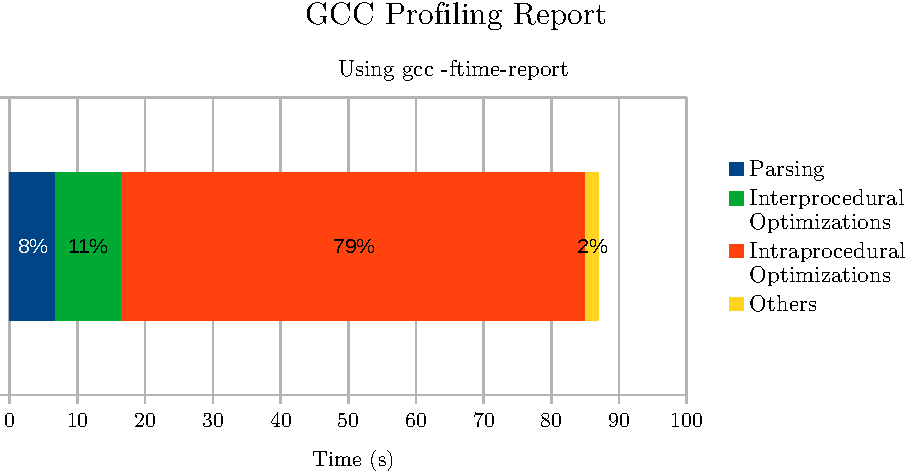
\includegraphics[scale=0.6]{figuras/profiling-crop.pdf}
	  \caption{Profiling GCC with \texttt{gimple-match.c}}
	  \label{fig:gcc_profiling}
\end{figure}

In GCC, all Intraprocedural Analysis are executed after IPA. When LTO is
enabled, that analysis is done in the LGEN stage, which already runs in
parallel when LTO is activated \cite{glek2010optimizing}. This inspired us to
transplant the LTO partitioner for per-file classical compilation instead of
threading the compiler, which would result in a faster development process.

Therefore, the main idea is to partition the TU into multiple partitions, and
compile them separately \textit{after} the Interprocedural Optimizations were
decided. Once each partition is compiled, we merge the compiled code into a
single object file, maintaining compatibility with the original build tools.

\subsection{Theoretical Maximum Speedup}

On Figure \ref{fig:gcc_profiling}, the compilation of \texttt{gimple-match.c}
takes $87s$, where $79\%$ is spent on Intraprocedural Optimizations, consuming
an relevant slice of the compilation time. If we assume that we can parallelize
this part with linear speedup, and round up the time taken in the
Intraprocedural part to $80\%$ (which is $\frac{4}{5}$), then we can calculate
the parallel time $T_p$ with $p$ processors as:

$$ T_p = \frac{1}{5} T_1 + \frac{4}{5p}T_1 = \frac{1}{5} \left( 1 + \frac{4}{p}
\right)T_1 $$
where $T_1$ is the serial time we measured. By the definition of speedup,
the maximum speedup archivable in the compiler is:

$$\lim_{p \rightarrow +\infty} \frac{T_1}{T_p} = \lim_{p \rightarrow +\infty}
\frac{T_1}{\frac{1}{5} \left( 1 + \frac{4}{p} \right)T_1} = \lim_{p \rightarrow
+\infty} \frac{5}{1 + \frac{4}{p}} = 5$$

Therefore, if we devise an mechanism to parallelize every Intraprocedural
Optimization, we can archive up to $5\times$ speedup when compiling individual
files.

\section{Our Proposal} \label{sec:work}

We propose a modification in the LTO engine to make it work \textit{without}
having the context of the \textit{entire} program. Once this   is done, we can
use the LTO partitioner engine to partition the file and compile then in
parallel, similarly to LTO.

Our approach differs from LTO mainly in how we handle the IPA.
LTO handles these optimizations with the context of the whole program, while
our approach will only have the context of the original TU.
This allows optimizations as good as they are in the \emph{classical
compilation} scheme while benefiting from the extra parallelism opportunity
available in the LTO's LTRANS stage.

In this section, we will first discuss the internals of some parts of GCC,
which we had to modify for our implementation to work. In Subsection
\ref{sec:gcc_driver}, we present how we modified the GCC driver to reconstruct
the output object file, required for maintaining compatibility building tools
such as Make. Then, in
Subsection \ref{sec:lto_partitioner} we present a short algorithm for making
the LTO partitioner work for our proposal. In Subsection
\ref{sec:partition_mask} we present a necessary change we had to do in our work
about how partitions are applied in GCC. In
Subsection \ref{sec:name_clash_resolution}, we explain how we solved the issue
of private symbols with the same name being promoted to global.
Then in Subsection \ref{sec:integration_jobserver}, we present an optional part
of our work about communicating with the GNU Make Jobserver to keep track of
used processors. And finally, we discuss why our proposal is still compatible
with the Reproducible Builds project in Subsection \ref{sec:repro_builds}.

\subsection{The \texttt{gcc} Driver}\label{sec:gcc_driver}

A large program can be written in several languages, with each of them having
its own compiler. From a compiler theory perspective, a compiler
translates a program from a language $A$ to another language $B$
\cite{dragonbook}. In GCC, it translates several languages to assembly
of some architecture (\textit{e.g.} x86). This means that
encapsulating code in object files, or linking these files in an executable, are
not tasks of the compiler. However, the user can launch \texttt{gcc -o binary
file.c} and get a working binary. That is because the binary \texttt{gcc} is
a \textit{driver}, and it will launch the
necessary programs for the user. In fact, this line launches three programs,
as illustrated in Figure \ref{fig:gnu_toolchain}.

Therefore, if we want our changes do not break the building scripts
(\textit{e.g.}, Makefile) used by most projects -- which is mostly launching
\texttt{gcc file.c -c} which creates an object file \texttt{file.o} -- we must
ensure that we create a single object file for each file, not multiple, as does
the LTO partitioner. Fortunately, we can rely on GNU \textit{ld} partial linking
for merging objects file into one. Therefore, the solution to this problem is:
\begin{enumerate}
	\item Patch the LTO \textit{partitioner} to communicate the location of
	each created assembly file (.s) to the \textit{driver}. This can be
	done by passing a hidden flag \texttt{-fadditional-asm=<file>}
	by the driver to the partitioner, which the last will write to. This file can also
	be replaced with a Named Pipe for better performance if needed.

	Then, the partitioner checks if this flag has been passed to the compiler.
	If yes, then a \textit{compatible version} of the driver is installed. If
	the partitioner decides to partition the TU, it should \textit{retarget}
	the destination assembly file and write the retargeted name to the
	communication file.

	\item Patch the driver to pass this hidden flag to the
	\textit{partitioner}, and also to check if this file exists. If not, this means
	that (1) the compiler is incompatible or (2) it has chosen not to partition
	the TU. In the first case, the driver should call the assembler to every
	assembly file generated, and call the linker to generate the expected
	final object file. In the second case, simply fallback to the previous
	compilation logic.
\end{enumerate}

Figure \ref{fig:gnu_toolchain_patched} illustrates the code flow after these
changes.  The execution starts in the highlighted node \textit{gcc}, which
calls the compiler (cc1) with the necessary flags to establish a communication
channel among the parts. The compiler then will partition the TU and forks
itself into several child processes, one for each partition.

Once multiple processes are created, the compiler will communicate its output
.s file, and the driver then launch the assembler (\textit{as}) to
generate several object files, to finally launch the linker (\textit{ld}) to
merge them all into a single object file.

%After these changes, a good way to check if the changes are working is to
%bootstrap the compiler with a single partition, but writing the output
%path into the created communication channel. Bootstrapping can be a resource
%intensive task; therefore this is an excellent opportunity to write automated
%tests covering every case necessary for the bootstrap. This may also expose
%some extreme cases, for instance, the C compiler being called to process macros
%in files of distinct languages.

\begin{figure*}
\tikzstyle{block} = [rectangle, draw, fill=white,
    text width=6em, text centered, rounded corners, minimum height=2em]
\tikzstyle{line} = [draw, -latex]

%\makebox[\textwidth][c]{
\scalebox{0.8}{
\begin{tikzpicture}[node distance = 2.4cm, auto]
    % Place nodes
    \node [block]                      (cc1_1) {cc1};
    \coordinate [right= of cc1]          (c);
    \node [block, right= of c,fill={rgb:black,1;white,2}]        (driver1) {gcc};
    \node [block, above= of c]                      (cc1_2) {cc1};
    \node [block, below= of c]                      (cc1_3) {cc1};
    \coordinate [above= of driver1]          (c2);
    \coordinate [below= of driver1]          (c3);
    \node [block, right= of c2]      (as2) {as};
    \node [block, right= of c3]      (as3) {as};
    \node [block, right= of driver1]       (ld) {ld};
    \coordinate [left= of cc1]          (fonte);
    \coordinate [right= of ld]    (bin);

    % Draw edges
    \draw[->]    (driver1.west)    -- (cc1_1.east) node[midway, above] {\texttt{-fadditional-asm=<file>}};
    \draw[->]    ([xshift=+0.5cm]cc1_2.south) -- ([xshift=-0.5cm]driver1.north) node[midway, above, sloped] {Generates .s file};
    \draw[->]    ([xshift=+0.5cm]cc1_3.north) -- ([xshift=-0.5cm]driver1.south) node[midway, above, sloped] {Generates .s file};

    \draw[->]    (cc1_1.north)    -- ([xshift=-0.5cm]cc1_2.south) node[midway, above, sloped] {Forks};
    \draw[->]    (cc1_1.south)    -- ([xshift=-0.5cm]cc1_3.north) node[midway, above, sloped] {Forks};

    \draw[->]    ([xshift=+0.5cm]driver1.north)  -- (as2.south) node[midway, above, sloped] {Assemble received .s};
    \draw[->]    ([xshift=+0.5cm]driver1.south)  -- (as3.north) node[midway, above, sloped] {Assemble receibed .s};
    \draw[->]    (driver1.east)  -- (ld.west) node[midway, above, sloped] {Links};

%    \draw[->]    (cc1.east)    -- (as.west)       node[midway, above] {Assembler File};
%    \draw[->]    (cc1.east)    -- (as.west)       node[midway, above] {Assembler File};
%
%    \draw[->]    (cc1.east)    -- (as.west)       node[midway, below] {(.s)};
    \draw[->]    ([xshift=+0.5cm]as2.south)     -- (ld.north)       node[midway, above, sloped] {Object File};
    \draw[->]    ([xshift=+0.5cm]as3.north)     -- (ld.south)       node[midway, below, sloped] {Object File};
%    \draw[->]    (fonte.west)  -- (cc1.west)      node[pos=0, above] {Source File};
%    \draw[->]    (fonte.west)  -- (cc1.west)      node[pos=0, below] {(.c)};
    \draw[->]    (ld.east)     -- (bin.west)      node[pos=1, above] {\texttt{file.o}};
\end{tikzpicture}
}
%}%
\caption{Interaction between the \textit{driver}, the \textit{compiler}, and other tools
after our changes}
\label{fig:gnu_toolchain_patched}
\end{figure*}

\subsection{Adapting the LTO Partitioner}\label{sec:lto_partitioner}

In GCC, a TU is represented as a callgraph. Every function, global variable, or
clones (which may represent a function to be inlined) is represented as nodes
in a callgraph. If there is a function call from $f$ to $g$, or there is a
reference to a global variable $g$ in $f$, then there is an edge from $f$ to
$g$. This means that TU partitioning can be represented as a \emph{graph
partitioning} problem.

When LTO is enabled and GCC is in the WPA stage, the body of these nodes
is not present, just a \textit{summary} of them (\textit{e.g.} the size
in lines of code it had). This is done to save memory. However,
when LTO is disabled, the function body is present. Therefore,
the LTO WPA engine must be further patched to expect that the function
body is present when analyzing the program. 

Then comes the partitioner algorithm \textit{de facto}. In LTO, GCC tries to
create partitions of similar size, and always try to keep adjacent nodes together.
However, we devised an partitioning algorithm for our tests which only keeps
together nodes which are \textit{required} to be in the same partition. Therefore,
we do not focus on partition balance, although we did implement a very simple
partition merging logic for some balance.

This partitioning algorithm works as follows: for each node, we check if it is
a member of a COMDAT \cite{comdat} group, and merged it into the same
partition. We then propagate outside of this COMDAT group; checking for every
node that may trigger the COMDAT to be copied into other partitions and group
them into the same partition. In practice, this means to include every node hit
by a Depth-First Search (DFS) from the group to a non-cloned node outside of
the group.  Algorithm \ref{alg:comdat} presents a pseudocode of this process.
Most of this process is already present from the COMDAT dependency algorithm
from LTO.  We added the logic to expand the partition side if a duplicated
symbol is encountered, adding further non-duplicated symbols in to
the boundary, as we illustrate in Figure \ref{fig:comdat_frontier}. Notice how
$v_{16}$ is not added to the frontier, as is called by $v_{14}$, the symbol marked
as duplicated.

\begin{algorithm*}
\caption{Partition the callgraph into multiple partitions for parallel compilation}
\begin{algorithmic}
\State{Partitions $ds$} \Comment{Hold partitions. Can be implemented with Union-Find.}
\Procedure{lto\_merge\_comdat\_map}{Callgraph $G$} \Comment{To be called by the LTO partitioner.}
	\State{Initialize $ds$} \Comment{Initialize one partition per node. Partitions will be constructed by merging other partitions.}
	\For{each symbol of $G$ \textbf{as} $v$}
		\If{$v$ belongs to a COMDAT group}
			\State{merge\_comdat\_nodes($v$, partition of $v$)}
		\EndIf
		\State{merge\_contained\_symbols($v$, partition of $v$)}
	\EndFor
	\State{balance the partitions in $ds$}
	\State{build LTRANS partitions object \textbf{from} $ds$}
\EndProcedure

\Procedure{merge\_comdat\_nodes}{node $v$, Partition $set$} \Comment{Merge the COMDAT group and its frontier.}
	\If{$v$ is marked}
		\Return
	\EndIf
	\State{mark $v$}
	\If{$v$ belongs to a COMDAT group}
		\For{every node in the same COMDAT group of $v$ \textbf{as} $w$}
			\State{unite partition of $w$ with partition $set$}
			\State{merge\_comdat\_nodes($w$, $set$)}
		\EndFor
	\EndIf
	\If{$v$ belongs to a COMDAT group \textbf{or} $v$ is a duplicated symbol}
	\State{}
	\Comment{If $v$ is duplicated and not member of COMDAT group, we need to reach to an non-duplicated symbol to add to the frontier.}
		\If{$v$ is a function}
			\For{every caller of $v$ \textbf{as} $u$}
				\If{calledge $(u, v)$ is inlined \textbf{or} $v$ is a duplicated symbol} \Comment{Same as above.}
					\State{unite partition of $u$ with partition $set$}
					\State{merge\_comdat\_nodes($u$, $set$)}
				\EndIf
			\EndFor
% TODO: This is a little different than what is implemented. Check if this is
% really correct.
\Comment{thunk functions adjust their object \texttt{this} pointer before calling the function}
			\If{$v$ is a thunk function \textbf{and} $v$ is not inlined anywhere}
				\For{every callee of $v$ \textbf{as} $w$}
					\State{unite partition of $u$ with partition $set$}
					\State{merge\_comdat\_nodes($u$, $set$)}
				\EndFor
			\EndIf
		\EndIf
		\Comment{Look at all nodes refering $v$, and add them to the COMDAT partition as well}
		\For{every node referring $v$ \textbf{as} $u$}
			\State{unite partition of $u$ with partition $set$}
			\State{merge\_comdat\_nodes($u$, $set$)}
			\If{$u$ is a duplicated symbol} \Comment{If $v$ is a duplicated symbol, we must reach an non-duplicated symbol for the frontier}
				merge\_comdat\_nodes($u$, $set$)
			\EndIf
		\EndFor
	\EndIf
\EndProcedure
\Procedure{merge\_contained\_symbols}{node $v$, Partition $set$}
	\For{every node contained in $v$ \textbf{as} $u$}
		\State{unite partition of $u$ with partition $set$}
	\EndFor
\EndProcedure
\end{algorithmic}
  \label{alg:comdat}
\end{algorithm*}

\begin{figure}
\centering
	 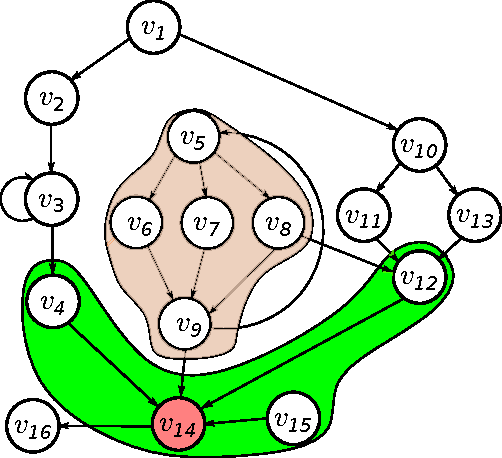
\includegraphics[scale=0.7]{figuras/comdat_frontier.pdf}
	  \caption{Example of callgraph, in beige being represented the COMDAT group,
	  in green the COMDAT frontier, and in red the cloned nodes.}
	  \label{fig:comdat_frontier}
\end{figure}

At first, we also did this process for private functions to avoid
promoting them to public, once external access would be necessary if they go
into distinct partitions. However, results showed that this has a strong
negative hit in any parallelism opportunity.

For grouping the nodes together,
we used a Union Find with Path Compression, which yields an attractive
computational complexity of $O(E + N \lg^*N)$ to our partitioner, where $N$ is the
number of nodes and $E$ is the number of edges in the callgraph \cite{feufiloff}.

Once the partitions are computed, we need to compute its \textit{boundary}.
If function $f$ calls $g$, but they were assigned into distinct partitions,
then we must include a version of $g$ in $f$'s partitions without its body,
then check if $g$ is a private function. If yes, then $g$ must be promoted
to a public function. There is also extra complexity if a version of $g$
is marked to be inlined in $f$, which means that its body has to be
streamed somehow. Fortunately, most of this logic is already present
in LTO and we could reuse them. However, some issues were found
when handling inline functions and global variables marked as part
of the boundary. First, some functions marked to be inlined into 
functions inside the partition were incorrectly marked to be removed.
We fixed that by checking if a marked to be removed function is inlined
into a function inside the boundary.
Second, being variables marked as in the boundary (and therefore
not in the partition) not being correctly promoted to external.
We further fix that by checking if there are references to that variable
through other partition, and in this case we promote them to global.

Furthermore, there were some issues concerning how GCC handles
partitions, which we discuss in the next subsection.

\subsection{Applying a Partition Mask}\label{sec:partition_mask}

Once partitions are computed, the only presented way to apply it
(\textit{i.e.}, remove every unnecessary node from the TU) was to reload the
compiler and let it load the phony object files. The issue is that these
objects are not available in our project because we are not running in LTO
mode. We developed another method for this.
We used the Unix \textit{fork} function to spawn a child process, and then
we implemented our own method to apply the partition without having to load
these phony object files. Fortunately, this consisted
of four cases:
\begin{itemize}
	\item \textit{Node is in partition}: nothing has to be done.
	\item \textit{Node is in boundary, but keep its body}: we mark that this function
	is available in other partitions, but we do not release its body or
	data structures.
	\item \textit{Node is in boundary}: we mark this mode as having its body removed,
	but we never actually remove it. This is because the node may share the
	body contents with another node in the partition. We then remove
	every edge from its functions to its callees, all references to variables,
	the content of the Dominator Tree, and also its Control-Flow Graph. This
	is now a function which this partition only know that it exists.
	\item \textit{Node not in boundary}: we remove the node and all its content.
\end{itemize}

After this, it retargets the output assembly file to another file private to
this partition and writes a pair (\textit{partition number, path to file}) into the
communication file, which the driver will read in the future. The partition
number is important to guarantee that the build is reproducible, as we will
discuss later.

It is also important that some early step in the compiler does not emit
assembly too early, such as were the case of the gimplifier in GCC, or else the
output file will be incomplete. These cases could be easily detected by using
an breakpoint and flushing the assembler output file before retargeting the new
assembler output file.

Once the partition is applied to the child process, and the output file has
been communicated to the driver, it can continue with the compilation. It
should be running in parallel now by the number of partitions.

\subsection{Name Clash Resolution}\label{sec:name_clash_resolution}

In LTO, if there are two promoted symbols to global with the same (mangled) name, a
straightforward way to fix that is to increment a counter for each clashed
symbol. This is possible because LTO has the context of the entire program,
which we do not. Therefore, we need another way of fixing it.

Two naive approaches would be to select a random integer and append to the
function's name, or append the memory address of the function object to the
function's name.  Both of them breaks bootstrap \cite{bootstrap}, the first
because output functions will have distinct names on every new compilation. The
second because stage 1 compiles with \texttt{-O0} and stage 2 with
\texttt{-O2}, which changes the memory address of the functions between these stages.

Our solution is to use a crc32 hash of the original file and append it to the
function's name.  There is still a tiny probability of name clash with this
approach, however, we did not find any on our tests.

\subsection{Integration with GNU Make Jobserver}\label{sec:integration_jobserver}

GNU Make can launch jobs in parallel by using \texttt{make -j}.  To
avoid unnecessary partitioning and job creation when the CPU is at 100\% usage,
we have also implemented an integration mechanism with GNU Jobserver
\cite{posixjobserver}.  The implementation is simple: we query the server for
an extra token. If we receive the token, then it means that some processor is
available, and we can partition the TU and launch jobs inside the compiler.
Else, the processor workload is full, and it may be better to avoid
partitioning altogether.

However, for a program to be able to communicate with the jobserver, it should
be launched with a prepended \texttt{+} character (\textit{e.g.} $\texttt{+gcc
-c file.c}$), and therefore it is not so straightforward to use this mode on
existing projects.

\subsection{Relationship with Reproducible Builds}\label{sec:repro_builds}

One interesting point of Open Source is that it can be verified by everyone.
However, very often these projects are distributed in a binary form to the
users, removing from them the burden of this process. But nothing avoids that a
malicious developer modifies the codebase \textit{before} the distribution
(\textit{e.g.} inserting a backdoor), and claiming that he/her got a distinct
binary because his/her system is different from the user.

The Reproducible Builds project aims to solve that issue by providing a way to
reproduce the released binary from its source. Some software needs to
be patched to work with Reproducible Builds, for instance,
to not contain some kind of build timestamp, and so on. A build
is called \textit{reproducible} if given the same source code and build
instructions, anyone can recreate a bit-perfect version of the distributed
binary \cite{reproducible_builds}.

To keep compatibility with this project, we must ensure that our compiler
always outputs the same code with a given input. The input is not only
the source file itself but also the flags passed to it.

We claim that our modification still supports the Reproducible Builds because
of the following reasons:

\begin{itemize}
	\item No random information is necessary to solve name clashing.
	\item Given a number of jobs, our partitioner will always generate
	the same number of partitions for a certain program, always with the same content.
	\item Partial Linking is always done in the same order. To ensure that,
	we communicate to the driver a pair (\textit{partition number, path to file}),
	and we sort this list using the partition number as the key.
	\item No other race conditions are introduced, as we rely on the quality of
	the LTO implementation of the compiler.
\end{itemize}

However, there is one point of concern, which is the Jobserver Integration.  If
the processor is already in 100\% usage, we avoid partitioning at all and
proceed with sequential compilation. This certainly changes accordingly to the
processor usage of the machine during the build, therefore the build is not
guaranteed to be reproducible if this option is enabled. This is not an issue
if the number of jobs is determined beforehand.

\section{Methods}\label{sec:methods}

We ensure the correctness of our changes by (1) bootstrapping GCC; (2) ensure
that the GCC testsuite was passing; and (3) compiling random programs generated
with \textit{csmith} \cite{csmith} and ensure that the correct result was
found. These tests were done with 2, 4, 8 and 64 parallel jobs, with minimum
partitioning quota of $10^3$ and $10^5$ instructions.

For the time measurements, all points represent the average of collected
samples, with errorbar representing a $95\%$ confidence interval.  Our test
files consisted of preprocessed source files from GCC, which compiles without
external includes. We collected $n = 15$ samples for every one of these files.
For the projects, we collected $n = 5$ samples because compilation is a
computer intensive task. We made sure that in every test, \texttt{-g0} was
passed for fairness, once in the current state we do not eliminate debug
symbols that are assigned to other partitions, which if enabled imposes an
unfair overhead that does not exist on the sequential version.

Tests were mainly executed in two computers, which are represented
in Table \ref{table:machines}. The graphic caption specifies where the test
was run.

For the tests regarding the compilation of entire projects, we used the Opteron
machine with make -j64 as the baseline and then enabling 8 internal threads in
the compiler. We then enabled the jobserver integration feature and let it use
how many threads as GNU Make allowed.

The version of GCC used in the tests is available in the \texttt{icpp2021}
branch of \texttt{git://gcc.gnu.org/git/gcc.git}, with hash \texttt{450b006f3}.

%We ensure the correctness of our changes by:
%\begin{enumerate}
%	\item Bootstraping GCC with the number of parallel jobs as
%	2, 4, 8 and 64, with minimum partitioning quota of $10^3$ and $10^5$
%	instructions. We found issues with regard 
%
%	\item Run the GCC testsuite, which we noticed that all tests related to the debug
%	symbols were failing. However, if \texttt{-g0} is passed, no debug symbol is created,
%	and the bug related to this issue is never triggered. The reason behind this is
%	because our partition applier do not remove the symbols associated with removed
%	nodes, resulting in unknown symbol being dumped into assembler.
%
%	\item Generated random programs with \textit{csmith} \cite{yang2011finding}. This found more complicated
%	bugs (for instance, long strings being output before the assembler file retarget),
%	which we fixed.
%\end{enumerate}

\begin{table}[]
\centering
\begin{tabular}{c|c|c|c|c|}
\cline{2-5}
                                      & No. Cores & No. Threads & RAM                                                    & Storage Dev. \\ \hline
\multicolumn{1}{|c|}{Core-i7 8650U}   & 4               & 8                 & \begin{tabular}[c]{@{}c@{}}8Gb\end{tabular} & SSD       \\ \hline
\multicolumn{1}{|c|}{4x Opteron 6376} & 32              & 64                & \begin{tabular}[c]{@{}c@{}}252Gb\end{tabular}   & HDD       \\ \hline
\end{tabular}
\caption{Machine specification of tests}
\label{table:machines}
\end{table}

\section{Results}\label{sec:results}

We first highlight some of our results in Table \ref{table:files}. On this
table, the autogenerated column means that this file is compiled to C++, and
then compiled into assembly by GCC. Furthermore, Figure
\ref{fig:gcc_all_files} shows the timings and speedups of compiling files with
Number of Instructions (insns) > $5\times 10^4$. We used the insns as a metric
instead of Lines of Code (LoC) as it better captures template-heavy code that
has to generate multiple functions for each argument type of the template from
the same input. In this figure, we can see that for large files, we mostly got
speedups in general. We managed speedups of up to a $2.4\times$ on Core-i7 when
compiling individual files with 8 threads, and up to $3.53\times$ on Opteron
6376 when with 64 threads. These speedup results is reasonably distant than
the linear optimal ($4.4$ if $p = 32$), so these results could be further improved.

We also notice that there is a file with $0.7\times$ speedup
(\textit{i.e}., a slowdown) named \texttt{brig-lang.c}. The reason for that is
the existence of a massive blob function that is appended to that file during
the compilation process (47261 insns, while the file itself has 55927 insns).
This was not observed in the remaining files. Since we partition the file by
functions and global variables, and this function consumes practically the
entirety of compilation time, we were not able to extract any meaningful
parallelism from this file.

%\begin{figure}
%\centering
%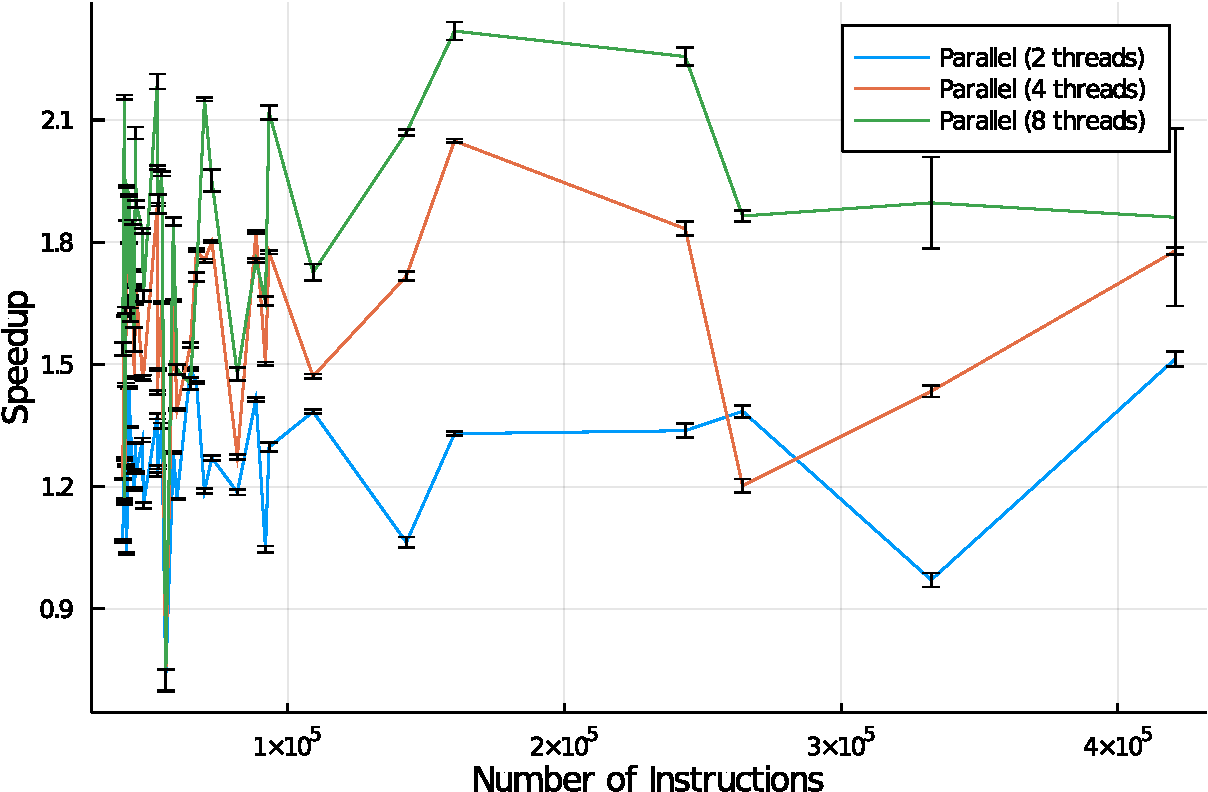
\includegraphics[scale=0.4]{figuras/times-speedup-crop.pdf}
%\caption{Speedups of selected files with 1, 2, 4 and 8 threads on Core-i7}
%\label{fig:gcc_speedups}
%\end{figure}
%
%\begin{figure}
%\centering
%	 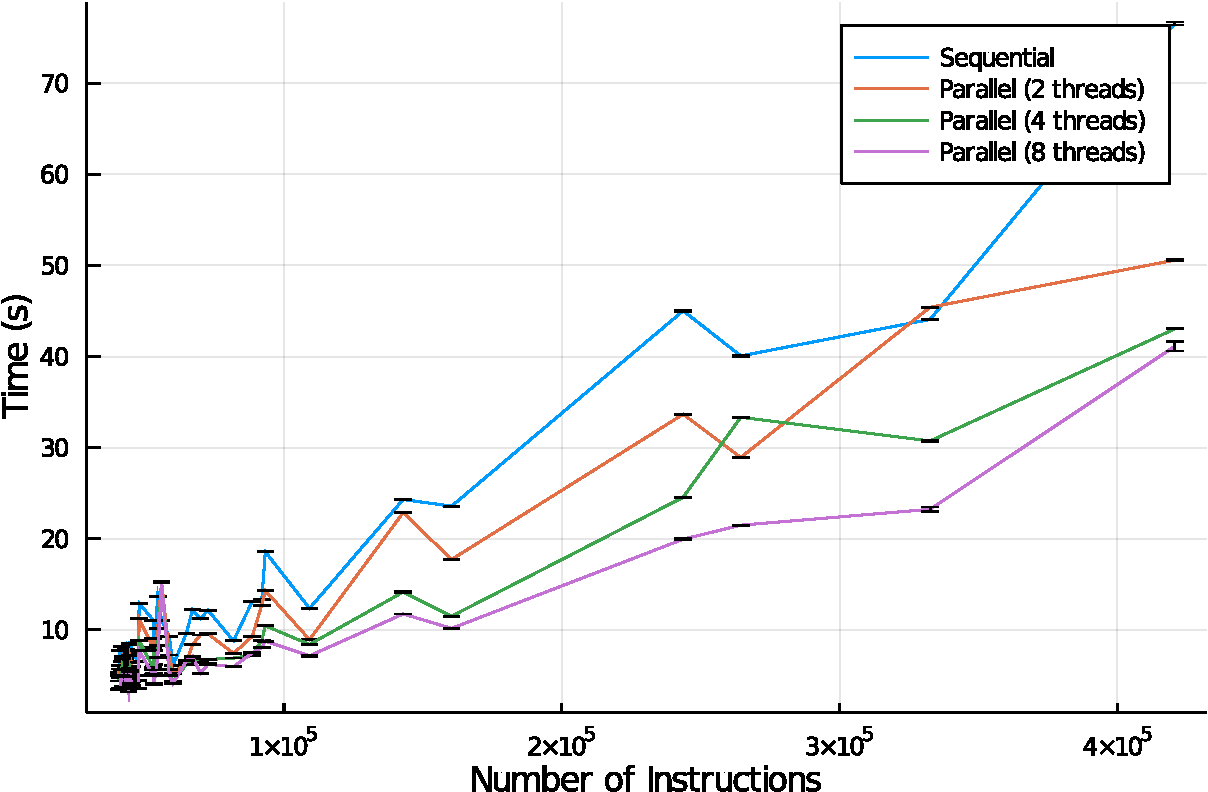
\includegraphics[scale=0.4]{figuras/times-insns-crop.pdf}
%	  \caption{Compilation of each file with 1, 2, 4, and 8 threads on
%	  Core-i7}
%	  \label{fig:gcc_all_files}
%\end{figure}

\begin{figure*}
\begin{minipage}[b]{0.5\textwidth}
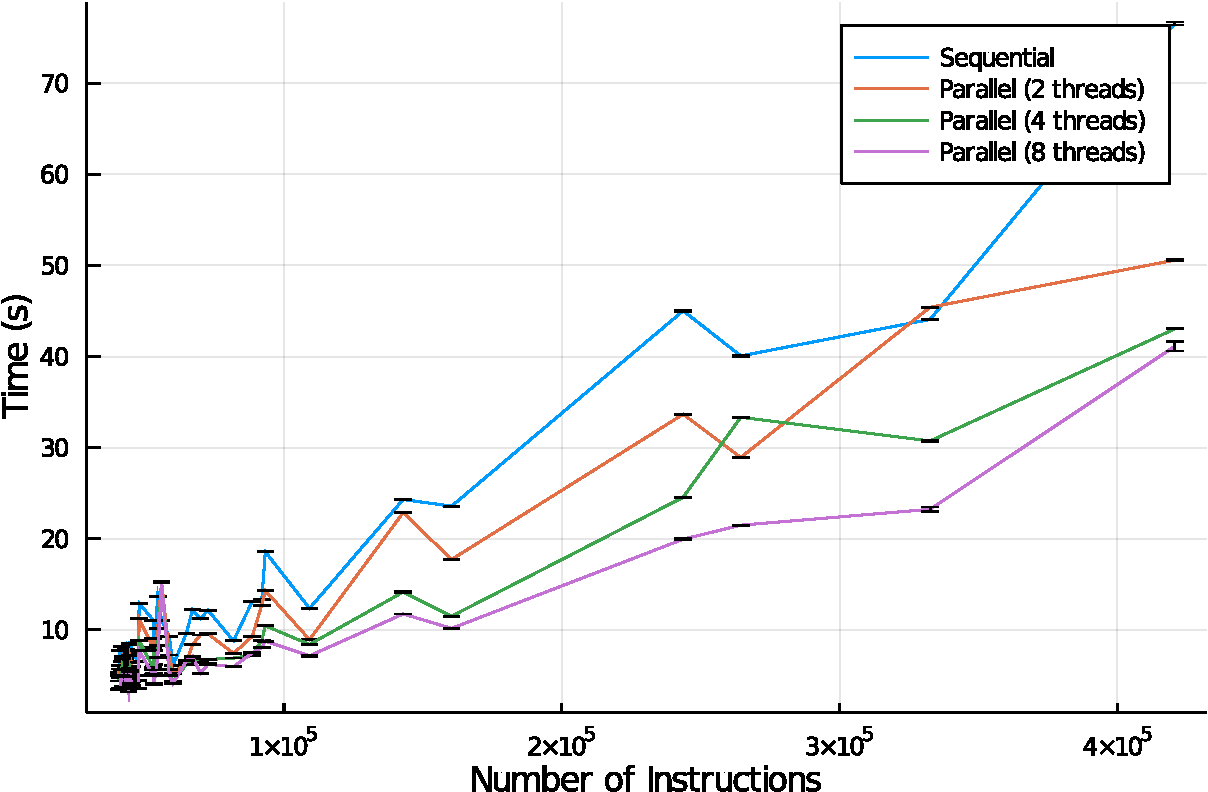
\includegraphics[scale=0.4]{figuras/times-insns-crop.pdf}
%\subcaption{A subfigure}
\end{minipage}%
\begin{minipage}[b]{0.5\textwidth}
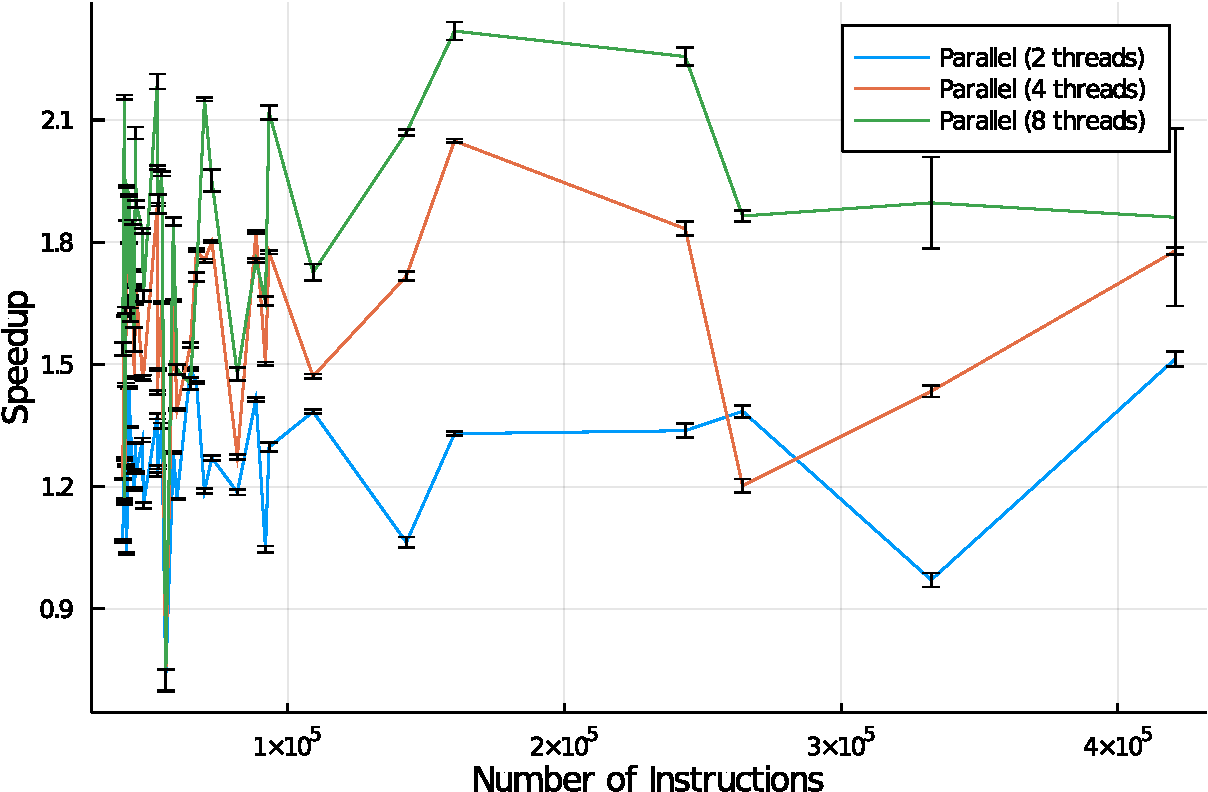
\includegraphics[scale=0.4]{figuras/times-speedup-crop.pdf}
%\subcaption{Another subfigure}
\end{minipage}%
\caption{Times and Speedups of selected files with 1, 2, 4 and 8 threads on Core-i7}
\label{fig:gcc_all_files}
\end{figure*}

We will now discuss how our proposed changes impact the overall compilation
time of some projects. For this, we run experiments compiling the Linux Kernel
5.8-rc6, Git 2.30.0, the GCC version mentioned in Section \ref{sec:methods}
with and without bootstrap enabled, and JSON C++, with commit hash
\texttt{01f6b2e7418537}. We selected those projects as they are very often used
on the Open Source community.  We have only enabled jobserver integration in
GCC and Git, because it is necessary to modify an absolute large number of
Makefiles for that (for instance, Linux has 2597 Makefiles).

In Figure \ref{fig:gcc_projects} we show our results. We ran this benchmark on a
64-threaded Opteron machine instead of the Quad-Core i7 machine, once we find
reasonable that our methodology would have better results on high core count
machines, and close to none improvement on low-core count machines.  We can
observe a near $35\%$ improvement when compiling GCC with bootstrap disabled,
$25\%$ when bootstrap is enabled, and $15\%$ improvement when compiling Git
compared to \texttt{make -j64} alone. Our jobserver implementation also
squeezed a small improvement in GCC compilation, but showed a massive slowdown
in Git. This is because Jobserver integration has interprocess communication
cost with Make, which is a problem if the size of the partitions is small.
Other than this, we seen no significant speedup or slowdown in these
other projects.

The most exciting result of these tests was the 35% speedup when compiling GCC,
which caught our attention. There must be some property in this project that
made our parallel compiler perform so well when compared to other projects.
Therefore, we executed one more experiment to profile how does the per file
parallelism behave specifically on GCC. We compiled GCC once more, registering
the timestamp of the beginning and the end of each file compilation. This
resulted in an interval graph, which we show in Figure
\ref{fig:analysis_classical}.  In this figure, it is clear that some automated
generated files simply bottleneck the entire compilation process. When we
enabled the internal threading feature as described above, it reduced the time
taken to compile these files, as illustrated in Figure
\ref{fig:analysis_classical_parallel}.  For instance, we were not able to
reproduce this behavior on the Linux Kernel, meaning that the compilation time is
evenly distributed across the files in this project.

Another interesting observation from both Figures \ref{fig:analysis_classical} and
\ref{fig:analysis_classical_parallel} is the high amount of serial steps when
compiling GCC until the high throughput compilation phase starts. This can be
attributed to GNU Autotools configuring the compiler for the environment of the
machine. Perhaps the configure part could be parallelized as well, and this
could improve several projects across the board, or replace this tool
altogether with another that can better handle parallelism.


\begin{table*}[]
\makebox[\textwidth][c]{
\begin{tabular}{l|c|c|c|c|c|c|c|c}
\cline{2-7}
                                       & \multicolumn{3}{c|}{Core-i7}     & \multicolumn{3}{c|}{Opteron 6376}                                                                & \multicolumn{1}{l}{}               \\ \hline
\multicolumn{1}{|l|}{File}             & Sequential & 8 Threads & Speedup & \multicolumn{1}{l|}{Sequential} & \multicolumn{1}{l|}{64 Threads} & \multicolumn{1}{l|}{Speedup} & \multicolumn{1}{c|}{Autogenerated} & \multicolumn{1}{c|}{LoC}  \\ \hline
\multicolumn{1}{|l|}{gimple-match.c}   & $76s$        & $31s$       & $2.4\times$     & $221s$                            & $66s$                             & $3.32\times$                         & \multicolumn{1}{c|}{yes} & \multicolumn{1}{c|}{$244320$}          \\ \hline
\multicolumn{1}{|l|}{insn-emit.c}      & $23s$        & $10s$       & $2.25\times$    & $97s$                             & $37s$                             & $3.53\times$                         & \multicolumn{1}{c|}{yes}  & \multicolumn{1}{c|}{$273482$}         \\ \hline
\multicolumn{1}{|l|}{tree-vect-stmt.c} & $11s$        & $5s$        & $2.14\times$    & $32s$                             & $13s$                             & $2.46\times$                         & \multicolumn{1}{c|}{no}    & \multicolumn{1}{c|}{$117285$}        \\ \hline
\multicolumn{1}{|l|}{brig-lang.c} & $10s$        & $15	s$        & $0.7\times$    & $29s$                             & $35s$                             & $0.8\times$                         & \multicolumn{1}{c|}{yes}    & \multicolumn{1}{c|}{$117087$}        \\ \hline
\end{tabular}
}
\caption{Speedup of highlighted files}
\label{table:files}
\end{table*}

%\begin{figure*}
%\begin{minipage}[b]{0.5\textwidth}
%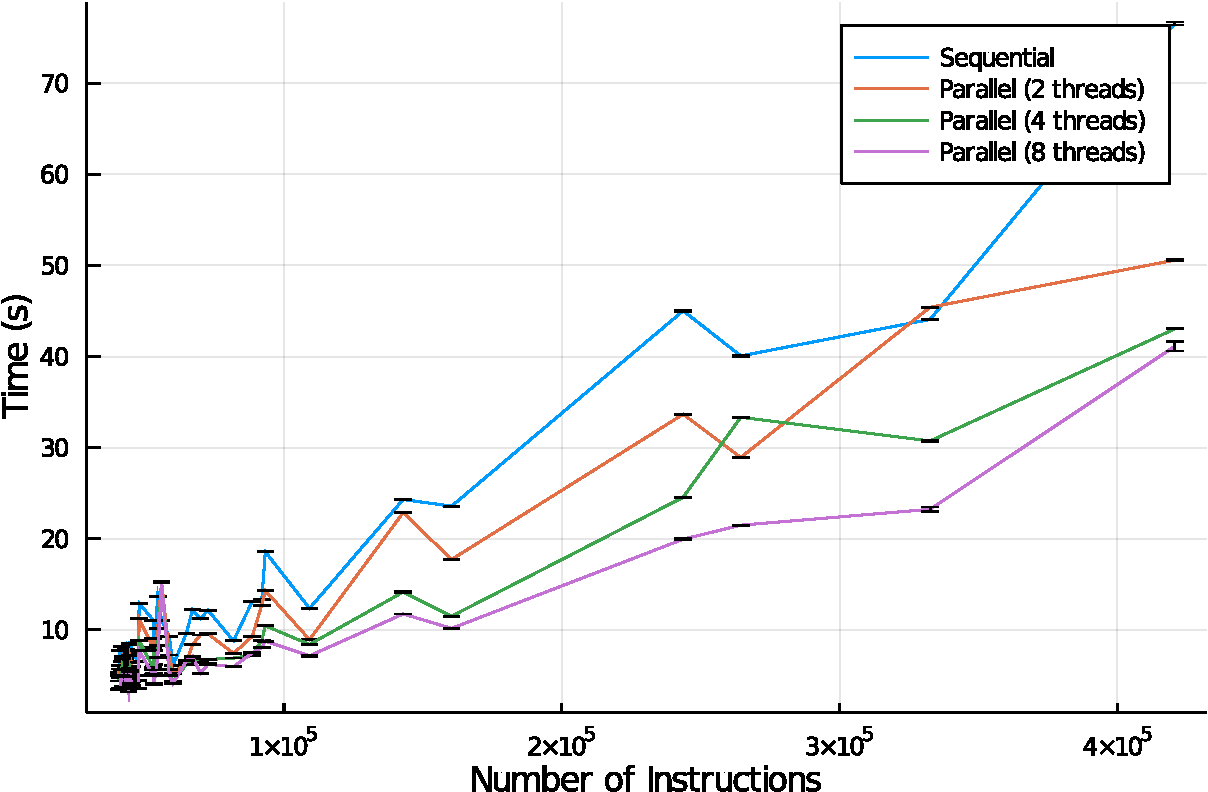
\includegraphics[scale=0.4]{figuras/times-insns-crop.pdf}
%%\subcaption{A subfigure}
%\end{minipage}%
%\begin{minipage}[b]{0.5\textwidth}
%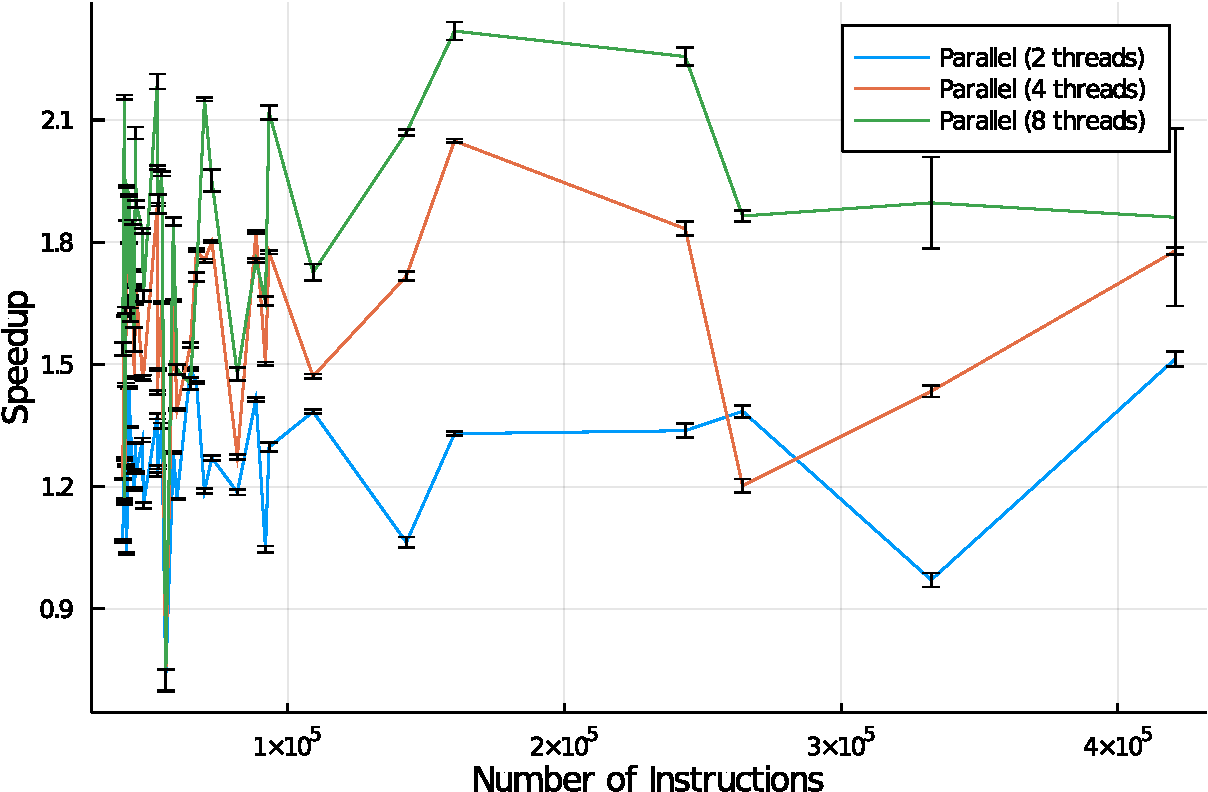
\includegraphics[scale=0.4]{figuras/times-speedup-crop.pdf}
%%\subcaption{Another subfigure}
%\end{minipage}%
%\caption{Times and Speedups of selected files with 1, 2, 4 and 8 threads on Core-i7}
%\label{fig:gcc_all_files}
%\end{figure*}

\begin{figure*}
\centering
	 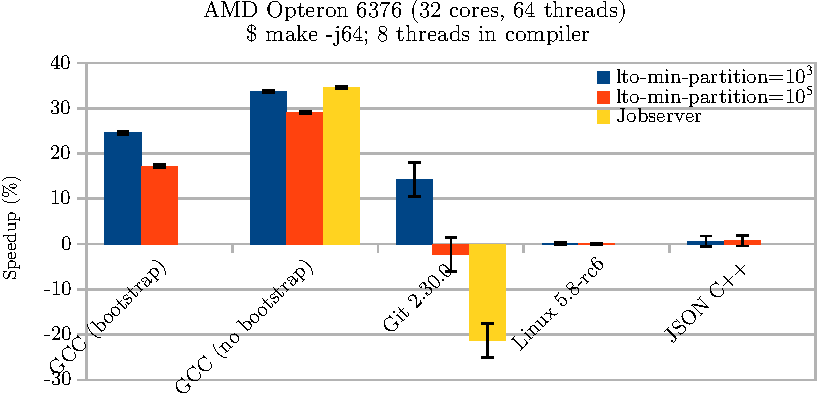
\includegraphics[scale=0.9]{figuras/experiment_projects_new-crop.pdf}
	  \caption{Compilation of some projects with 64 Makefile jobs and 8 threads in compiler in Opteron 6376}
	  \label{fig:gcc_projects}
\end{figure*}

\begin{figure*}[ht]
% \vspace*{-2cm}%
 \noindent%
% \hspace*{-2cm}%
    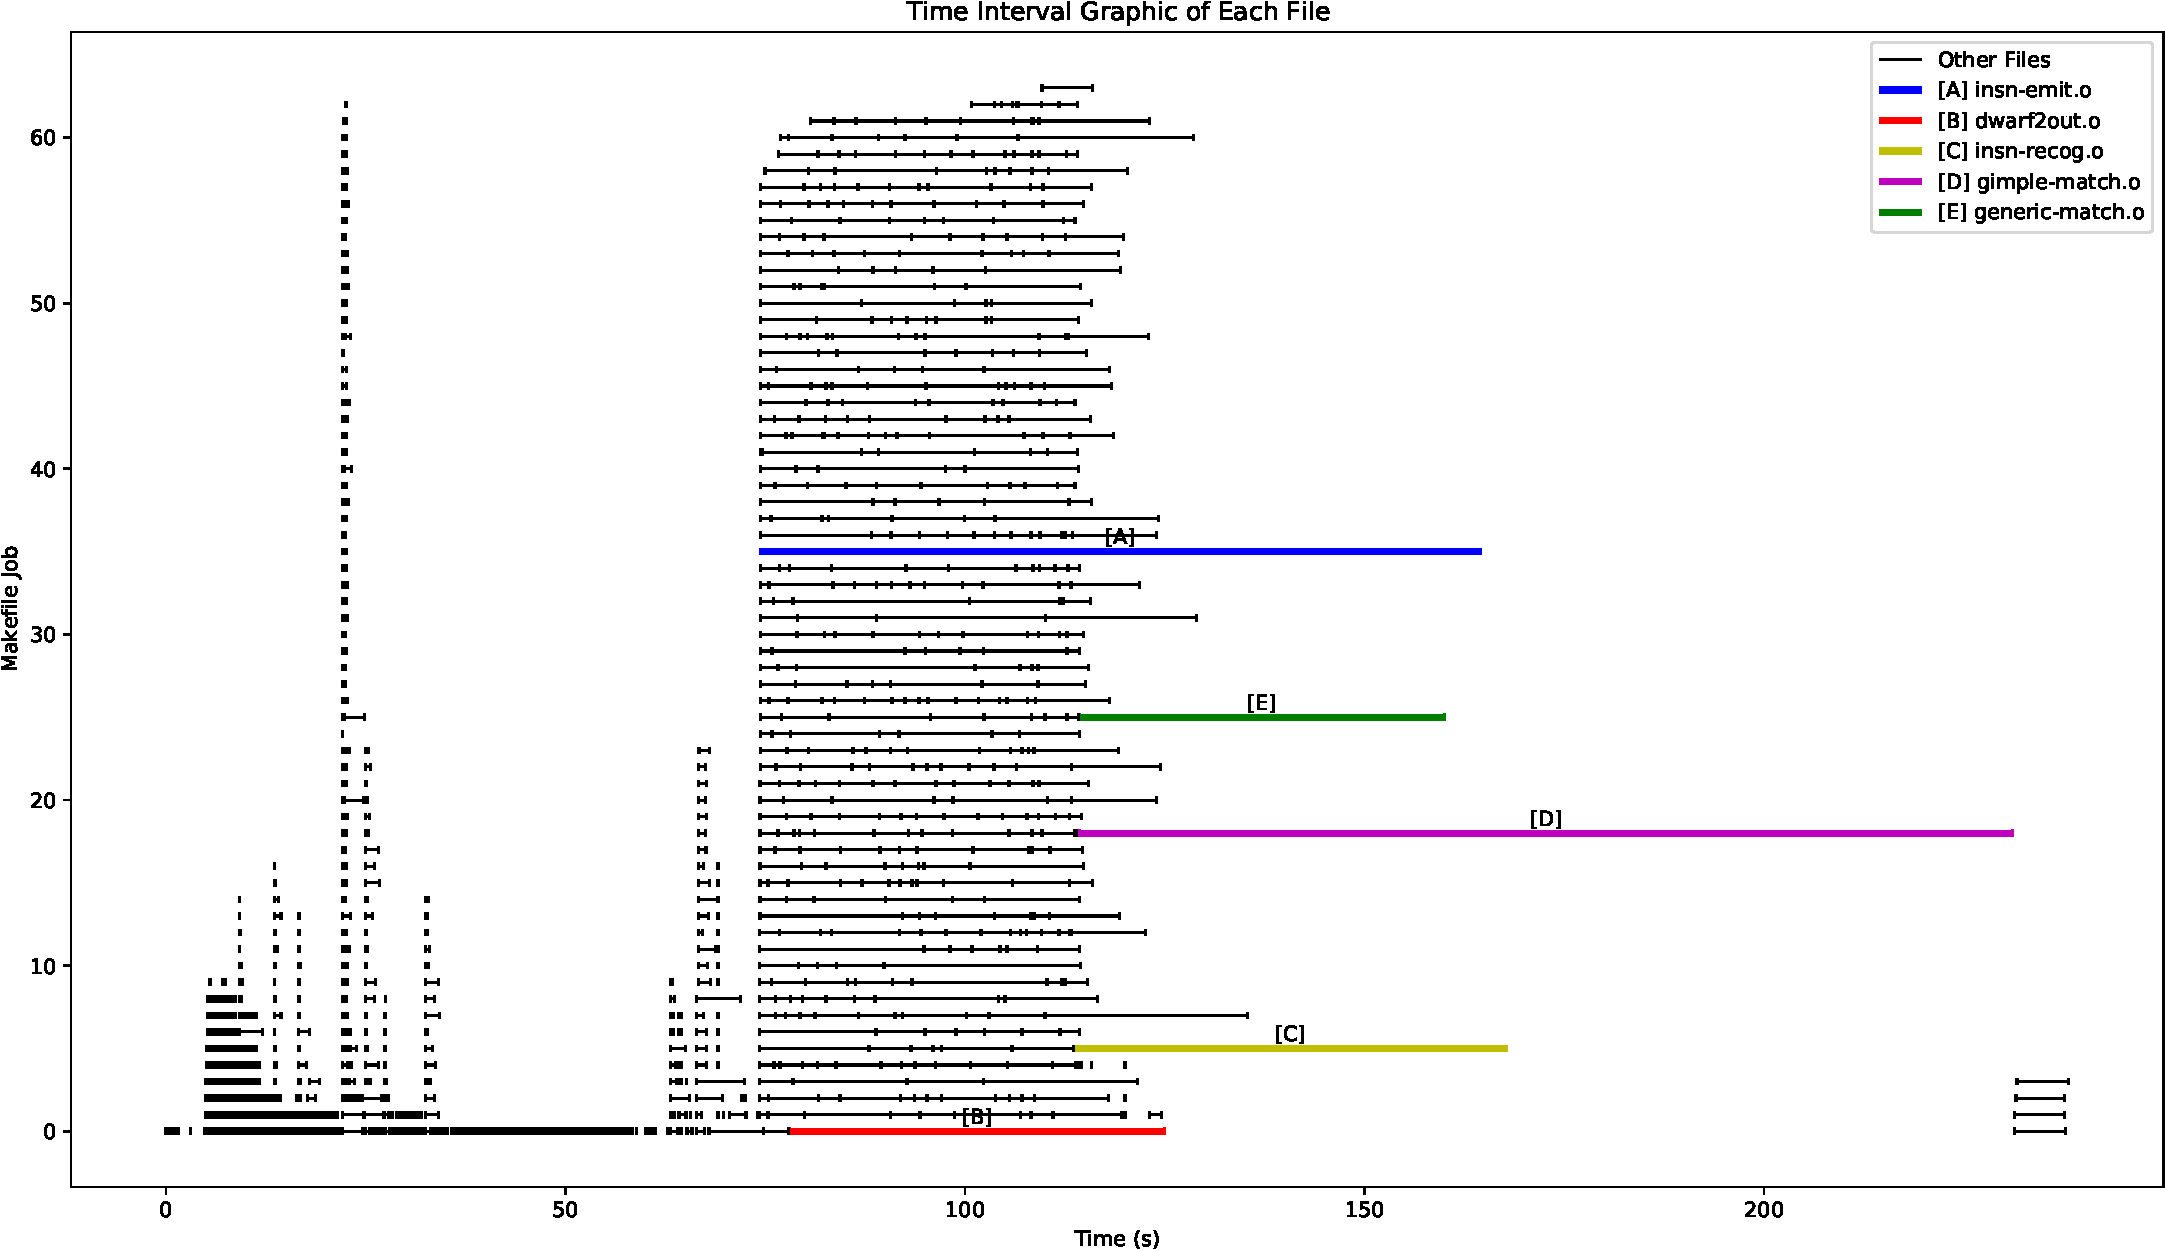
\includegraphics[width=0.76\paperwidth]{seq-crop.pdf}
    \captionof{figure}{Compilation time of GCC without our modifications}
    \label{fig:analysis_classical}
\end{figure*}
\vfill
\begin{figure*}[ht]
% \vspace*{-2cm}%
 \noindent%
% \hspace*{-2cm}%
    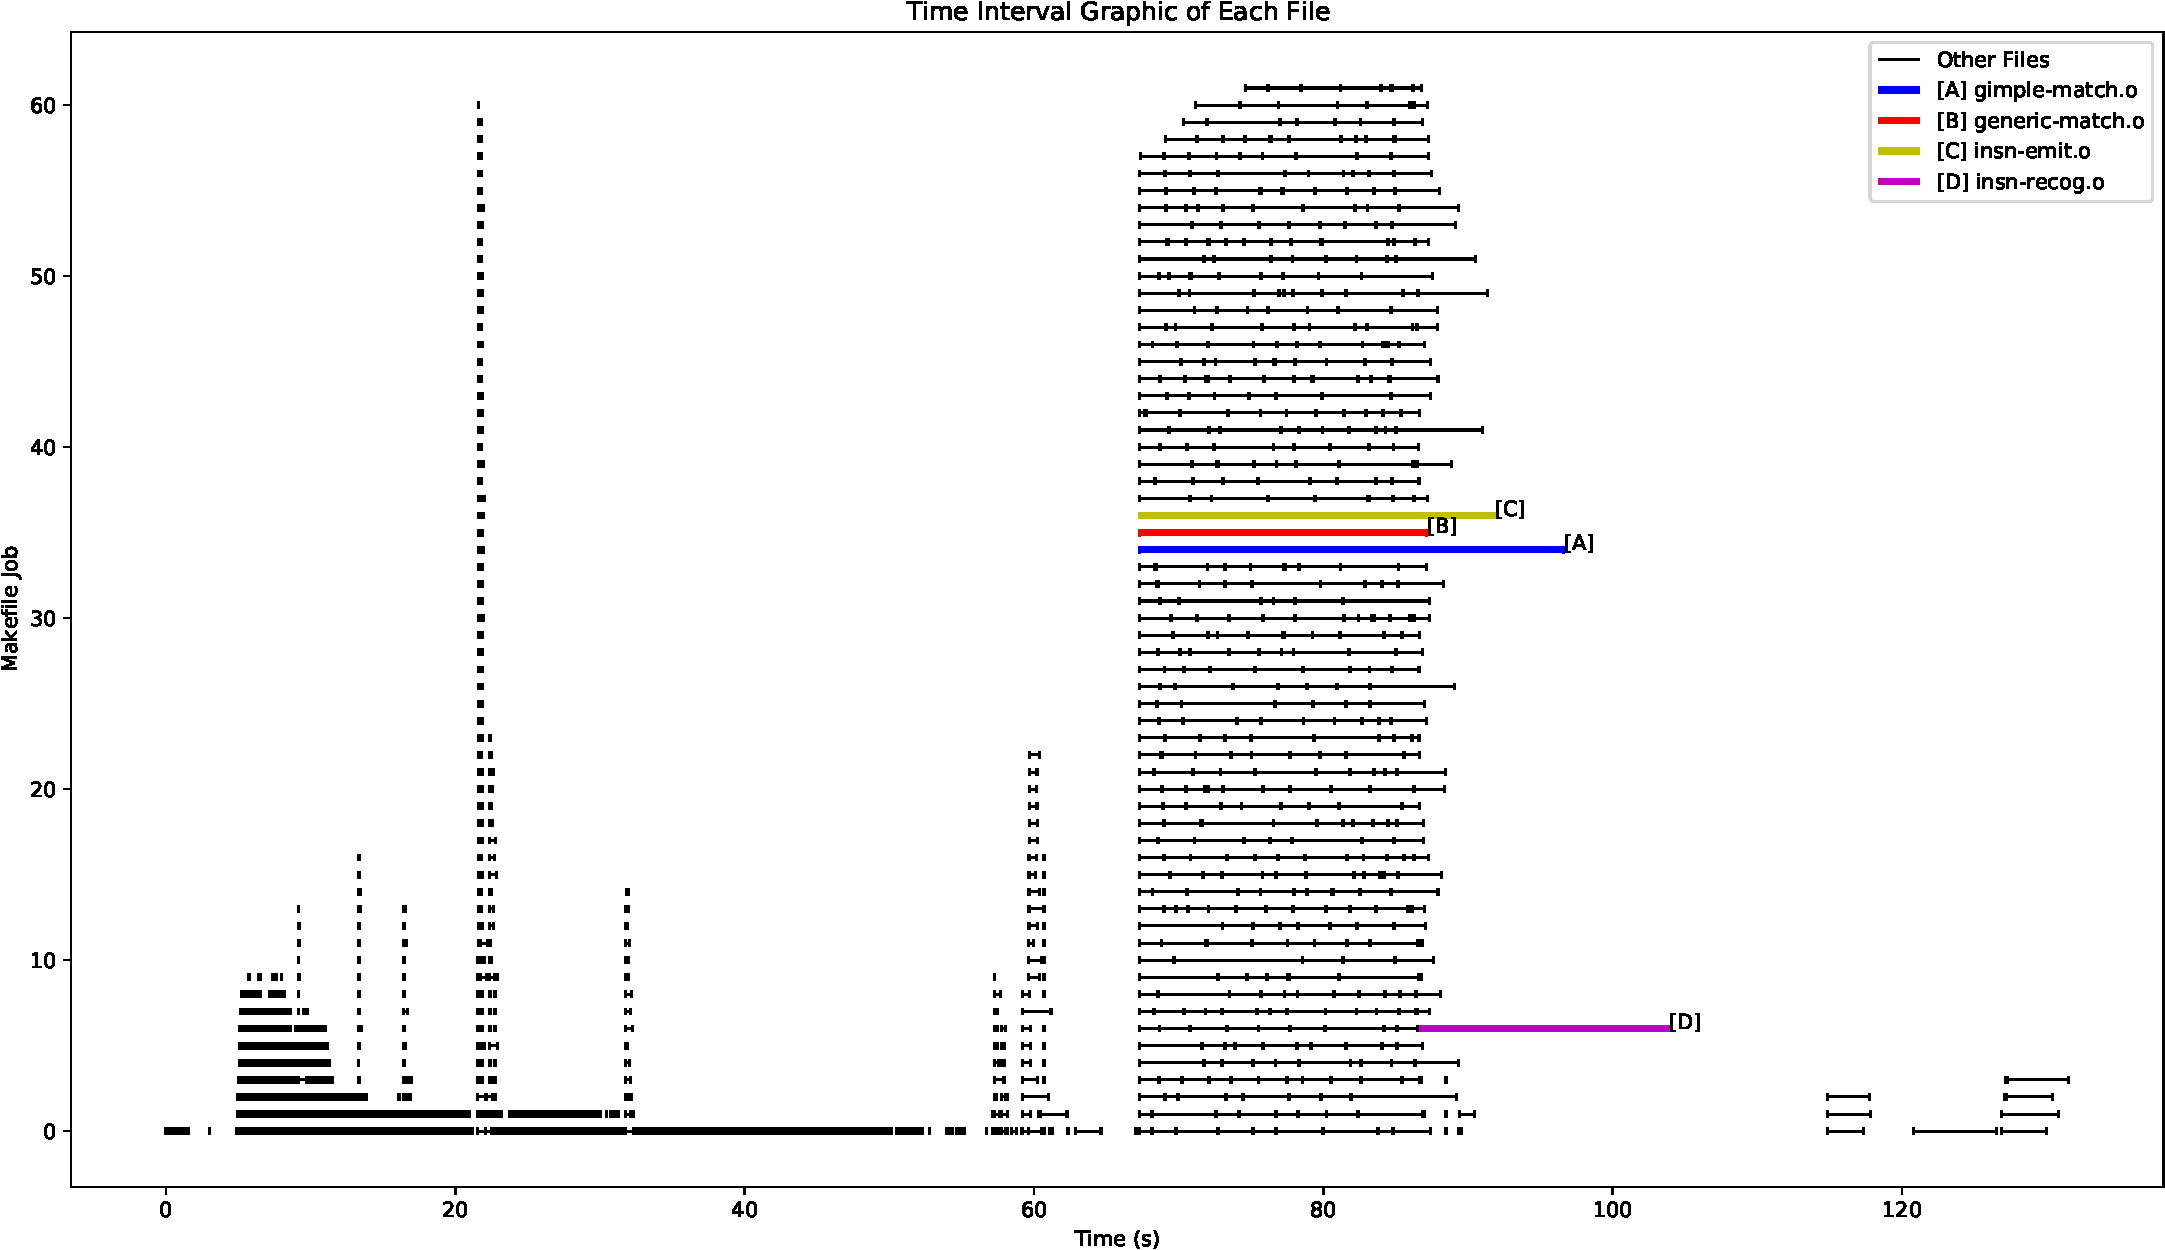
\includegraphics[width=0.76\paperwidth]{par-crop.pdf}
    \captionof{figure}{Compilation time of GCC, using 8 internal threads
	and partition if $\textit{Number of Instructions} > 10^3$}
    \label{fig:analysis_classical_parallel}
\end{figure*}
\section{Conclusions, Issues, and Future Works}\label{sec:future_works}

We have shown a tangible way of compiling files in parallel capable
of being implemented in industrial compilers, which resulted in
speedups when compiling single files in parallel, as well as some
speedup when compiling entire projects in manycore machines. 

Our main conclusion is that parallel file compilation is useful in two scenarios:
the existence of massive autogenerated blob files in
the project, which consumes a large amount of compilation time when compared to
the remaining files of the project, and (2) the number of files in the project
is not enough to fully populate the processors of the machine. This means that
our approach have some limitations, but results in decent speedups in some
cases. Else, our methodology performs as good as the default per-file compilation
parallelism.

Furthermore, there are several points in which our work can be improved.
First is by fixing the bugs which is already known. Mainly, the issue with our
partitioner that applier do not remove debug symbols associated with removed
nodes, resulting in duplicated symbols being dumped into the final assembly. This
result in several unnecessary writes to disk, which slows down the parallel
compilation process. This is an programming issue rather than a design flaw,
and therefore it is still fine as a proof of concept to support our claims.
Furthermore, this could be used in projects where LTO imposes an slowdown.
Johnson \textit{et al.} show some of these projects when presenting ThinLTO
\cite{thinlto}.

Second is by implementing a better load balancing algorithm to the project,
once we only kept its load balancing algorithm minimal to ensure that it works.
Using the LTO default partitioner as a base is a good start.

Third, try to develop a predictive model to decide if the input file is
a good candidate for parallel compilation. Figure \ref{fig:gcc_all_files} shows
a clear linear correlation between the expected number of instructions and time
(and maybe it is the best parameter), but it may be possible to (statically)
collect more information about the file for a better decision.

And fourth, try to avoid partial linking and symbol promotion altogether by
concatenating the generated assembly files, instead of linking every generated
assembly file into temporary object files. This should eliminate any possibility
that promoting symbols to public visibility may impact the binary performance
in a negative way.

We also would like to draw attention to LTO's WPA step, which still runs
sequentially. Parallelizing this step, which includes all IPA passes would
improve parallel compilation of projects across the board in both LTO mode and
in our work. Profiling shows us that $11\%$ of the compilation time is spent in
this mode, while our project parallelized $79\%$ of the compiler.

\bibliographystyle{ACM-Reference-Format}
\bibliography{sample-base}

\end{document}
%</manuscript|acmsmall|acmsmall-submission|acmlarge|acmtog|sigconf|authordraft|sigplan|sigchi|sigchi-a|acmsmall-conf>
